\section{Kameramodelle}
\subsection[DSLR Kamera - Aufbau]{DSLR Kamera - Aufbau\protect\footnote{\label{}vgl. http://bit.ly/2pnpDgL [Zugriff: 18.03.2018]}}
DSLR bedeutet Digital Single Lens Reflex und sind Spiegelreflexkameras mit digitalem Aufnahme Sensor. Beispiele für eine Spiegelreflexkamera sind die Canon EOS 60D oder die Canon EOS 70D. In der folgenden Abbildung wird der Aufbau einer DSLR Kamera dargestellt. Wie man in der Abbildung sehen kann, geht das Licht zuerst durch die Linse des Objektivs (1). Anschließend trifft das Licht auf den Schwingspiegel (2), welcher das Licht auf die Mattscheibe (5) reflektiert. Daraufhin verkleinert es die Sammellinse (6) auf die Größe des Suchers. Da das Bild noch spiegelverkehrt ist, spiegelt es das Pentaprisma (7) und kann so im Sucher (8) dann angezeigt werden. "Wenn man nun den Auslöser betätigt, klappt der Spiegel nach oben und gibt den Weg zum Schlitzverschluss (3) frei."\footnote{\label{}http://bit.ly/2pnpDgL [Zugriff: 18.03.2018]} Anschließend öffnet sich dieser Verschluss und das Licht fallt auf den Sensor (4). Zum Schluss wird das Bild abgespeichert.
\begin{figure}[H]
	\centering
	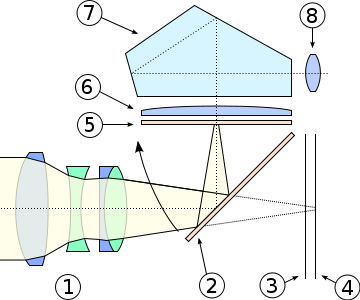
\includegraphics[width=0.6\textwidth]{abb13} 
	\caption{Aufbau einer DSLR Kamera}
\end{figure}
\subsection{Sensoren}
Heutzutage gibt es zwei Vorreiter im Bereich der Sensoren. Nämlich einerseits der CMOS-Sensor und andererseits den CCD Sensor. Welcher Sensor nun auch wirklich besser ist, und in welcher Kamera welcher Sensor eingebaut werden soll, ist jedoch noch umstritten.
\paragraph{CMOS-Chips}
\leavevmode \\
Die CMOS Sensoren haben den großen Nachteil, dass das Bild bei schnellen Bewegungen, etwa wie beim Filmen von fahrenden Autos, verzerrt dargestellt wird. Dies wird auch Rolling-Shutter-Effekt genannt. Bei dem Rolling-Shutter-Effekt schauen die vertikalen Linien so aus, als würden sie umfallen, was das Bild unbrauchbar machen kann.
\paragraph{CCD-Chips}
\leavevmode \\
Die CCD Sensoren haben zwar nicht das Problem mit dem Rolling-Shutter-Effekt, jedoch sind diese Sensoren lichtempfindlicher. Das bedeutet, dass wenn das Licht direkt ins Objektiv scheint, tritt der sogenannte Blooming-Effekt auf. Beim Blooming-Effekt wird das Bild von einem breiten weißen Streifen geteilt. Scheint Kunstlicht in das Objektiv, entstehen wandernde violette Streifen.
\subsection[Canon EOS 60D]{Canon EOS 60D\protect\footnote{\label{}vgl. http://bit.ly/2pnrmmy [Zugriff: 16.03.2018]}} Die Canon EOS 60D DSLR (Digital Single Lens Reflex) Kamera bietet einen 18 Megapixel APS-C CMOS Sensor mit einer Größe von 22,3 mm x 14,9 mm. Die Spiegelreflexkamera nimmt mit Full HD (1920 x 1080) auf, wobei standardgemäß mit 25 Bildern pro Sekunde aufgenommen wird. Die Auflösung wird meistens mit 1080p gekennzeichnet, wobei das p für progressive steht, also für die Vollbilder.
\subsection[Canon EOS 70D]{Canon EOS 70D\protect\footnote{\label{}vgl. http://bit.ly/2IxVmF2 [Zugriff: 16.03.2018]}} Die Canon EOS 70D bietet einen minimal größeren Sensor im Gegensatz zu der Canon EOS 60D. Die Größe des Sensors der Canon EOS 70D beträgt 22,5 mm x 15,0 mm. Die Sensorgröße einer Kamera ist entscheidend, da folgendes gilt: "Je kleiner der Sensor, desto geringer sind die Möglichkeiten, mit einer definierten Schärfentiefe zu arbeiten."
\footnote{\label{} Jörg Jovy, 2017, S. 136} Die Canon EOS 70D nimmt ebenfalls mit Full HD auf, wobei zu beachten ist, dass sie zusätzlich die Möglichkeit bietet, mit Intra-Frame oder Inter-Frame aufzunehmen. Bei Intra- oder Inter-Frames wird jedes Einzelbild komprimiert, das heißt, es kann auf jedes einzelne Bild zugegriffen werden
\footnote{\label{}vgl. https://www.univie.ac.at/video/grundlagen/intraframe.htm [Zugriff: 17.03.2018]}, was sich in der Post Production positiv widerspiegelt, da man keine Gruppen aus Bildern bearbeiten muss, sondern im Notfall jedes einzelne Bild bearbeiten kann. Weiters spielt bei der Wahl der richtigen Kamera, der Cropfaktor eine wichtige Rolle. "Je kleiner ein Sensor ist, desto kleiner ist auch der Bildwinkel des Objektivs."
\footnote{\label{}Jörg Jovy, 2017, S. 136} Das bedeutet, dass die Abbildungsfläche beschnitten wird, was einen engeren Bildausschnitt liefert und somit ein vergrößertes Bild darstellt. Was bei DSLR Kameras zu beachten ist, ist das sie einen Cropfaktor von 1,6 besitzen. So verhält sich durch den Cropfaktor von 1,6 ein Normalobjektiv mit 50mm Brennweite, wie ein leichtes Teleobjektiv mit 80mm Brennweite. 
Da die Canon EOS 70D einen minimal größeren Sensor besitzt, und die Möglichkeit bietet, mit Intra-Frames aufzunehmen, wurde die Canon EOS 70D DSLR Kamera für alle Aufnahmen verwendet.
\subsection[Objektive]{Objektive\protect\footnote{\label{}vgl. Jörg Jovy, 2017, S. 138f.}}
Die Brennweite eines Objektivs legt den Bildausschnitt fest. Die Brennweite wird in Millimeter angegeben und sagt aus, ob es sich um ein Normal-, Tele-, oder ein Weitwinkelobjektiv handelt.
Anhand der folgenden Abbildung kann man gut erkennen, dass ab 10 mm bis 24 mm Weitwinkelobjektive zum Einsatz kommen. Ein Normalobjektiv erkennt man daran, da es eine Brennweite von 50 mm besitzt und somit einen Bildwinkel von 46$^\circ$ hat. Teleobjektive finden ihren Einsatz bei 80 mm bis 200 mm. Anhand der Abbildung kann man gut den Unterschied zwischen der Brennweite von 10 mm und einem Bildwinkel mit 130$^\circ$, und einem Objektiv mit einer Brennweite von 200 mm mit einem 12$^\circ$ Bildwinkel erkennen. 
\begin{figure}[H]
	\centering
	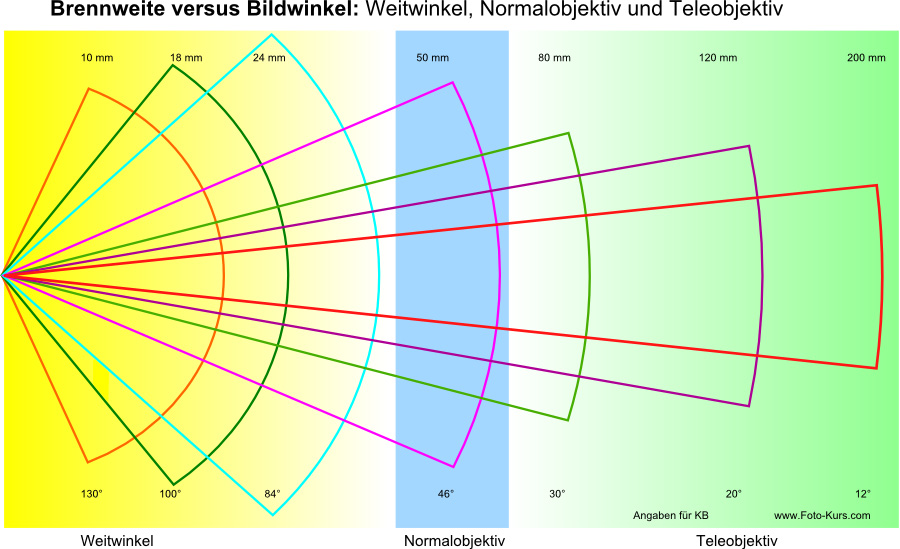
\includegraphics[width=0.7\textwidth]{abb1} 
	\caption{Brennweite und Bildwinkel}
\end{figure}
\begin{itemize}
	\item Normalobjektiv\footnote{\label{}vgl. Jörg Jovy, 2017, S. 196f.}
		\begin{itemize}
		\item Das Normalobjektiv entspricht im Grunde dem menschlichen Blickwinkel, und wird meist als natürlich empfunden. 
		\end{itemize}
	\item Weitwinkel
		\begin{itemize}
		\item Wie man auf der obigen Abbildung sehen kann, haben Weitwinkelobjektive einen breiten Bildwinkel, somit sieht man mehr vom Bild. 
		\end{itemize}
	\item Teleobjektiv
		\begin{itemize}
		\item Teleobjektive nehmen Objekte mit einem kleinen Blickwinkel aus großer Entfernung auf. Teleobjektive haben daher einen eher kleinen Schärfentiefenbereich, was sich beispielsweise für Interviews schlecht eignet. 
\end{itemize}
\end{itemize}
\paragraph{Schärfentiefe}
\leavevmode \\
"Die Schärfentiefe ist das Maß für den in einem Bild scharf abgebildeten Bereich." Der Sinn der Schärfentiefe ist, ein Objekt oder Motiv vom Hintergrund abzuheben, also es schärfer darstellen zu lassen als der Hintergrund.\newline
Die kann durch drei Parameter eingestellt werden:
\begin{itemize}
	\item Sensorgröße
	\item Blende
	\item Brennweite
\end{itemize}
Wie vorhin erklärt, hat der Sensor auch einen Einfluss auf die Schärfentiefe, nämlich je größer der Sensor ist, desto mehr Spielraum bietet sich.\newline
Je weiter die Blende geöffnet ist, desto geringer ist die Schärfentiefe. Zuletzt kann noch die Brennweite eingesetzt werden, um eine geringe Schärfentiefe zu erzeugen. Je näher man an ein Objekt heranzoomt, desto unschärfer wird der Hintergrund. \\ 
Bei allen drei Videos wurden Zoomobjektive verwendet. Zoomobjektive haben eine variable Brennweite, das heißt man muss sich nicht auf eine fixe Brennweite festlegen, sondern kann selbst entscheiden welche Brennweite man haben möchte. Bei dem Dreh der Videos kam das Canon Objektiv EF-S 18-135mm f/3.5-5.6 IS USM zum Einsatz. Durch das Zoomobjektiv war es möglich das Filmen flexibel zu gestalten. Beim Dreh des Interviews mit dem Abteilungsvorstand wurde die Brennweite nicht berücksichtigt und somit hat die nötige Schärfentiefe im Bild gefehlt. Dies wurde anschließend in der Post Production ausgebessert. Bei bei dem Tag der offenen Tür Video konnte mittels dem Wissen mittels der Brennweite die optimale Schärfentiefe erzielt werden.